\documentclass[12pt]{report}
\usepackage[francais]{babel}
\usepackage[utf8]{inputenc}
\usepackage[a4paper,left=2cm,right=2cm,top=2cm,bottom=2cm]{geometry}
\usepackage[pdftex]{graphicx}
\usepackage{float}
\usepackage{moreverb}
\usepackage{tikz-uml}
\usepackage{tikz-er2}

\usetikzlibrary{positioning}
\usetikzlibrary{shadows}
\tikzstyle{every entity} = [top color=white, bottom color=blue!30,
														draw=blue!50!black!100, drop shadow]
\tikzstyle{every attribute} = [top color=white, bottom color=yellow!20,
															draw=yellow, node distance=1cm, drop shadow]

\setlength{\parindent}{0.8cm}
\setlength{\parskip}{1ex plus 0.5ex minus 0.2ex}
\newcommand{\hsp}{\hspace{20pt}}
\newcommand{\HRule}{\rule{\linewidth}{0.5mm}}

\date{April 2017}

\begin{document}
	\begin{titlepage}

		\begin{center}

			
\includegraphics[scale=0.11]{images/logo-um.png}~\\[1.5cm]
			\textsc{\Large Faculté des Sciences de Montpellier}\\[2cm]
			\textsc{\Large Rapport de projet - Licence 2ème année}\\[0.5cm]
			\textsc{\Large Informatique - TER (HLIN405)}\\[0.5cm]
			\textsc{\Large 2016-2017}\\[1.5cm]

			\HRule \\[0.4cm]
			{ \huge \bfseries Jeu de cartes en ligne\\[0.4cm] }

			\HRule \\[2cm]
			
			\begin{flushleft}
				\begin{minipage}[b]{6cm}
					\large	\textsc{Beuret} Maëlle\\[0.5cm]
					\large	\textsc{Farajallah} Othmane\\[0.5cm]
					\large	\textsc{Rima} Bachar\\[0.5cm]
				\end{minipage}
			\end{flushleft}
			
				Début du projet : 18 janvier 2017
				
				Encadrant : P.Pompidor

			\vfill

			
\includegraphics[scale=0.3]{images/logo-fds.jpg}~

		\end{center}

	\end{titlepage}

	\tableofcontents

	\chapter*{Introduction}
	\addcontentsline{toc}{chapter}{Introduction}

		\section*{Présentation du jeu}
  	\addcontentsline{toc}{section}{Présentation du jeu}
  	Les Voyageurs de Kaeraly est un jeu de cartes coopératif en ligne. Le but des joueurs est de tuer le Loup Alpha. Pour cela, il leur faudra traverser différentes zones (forêt, rivière, plaine) à l'aide d'objets trouvés aléatoirement lors de leur voyage, en étant équipés d'armure ou d'armes, et utiliser des potions afin d'améliorer leurs statistiques d'attaque et de défense.

  	Inspiré des jeux de rôle sur table ainsi que des jeux de société tels que le Munchkin, nous avons eu l'idée de créer ce jeu en collaboration avec des illustrateurs venant de Suisse, de Roumanie et des Pays Bas, afin de partager l'expérience d'un jeu de société à distance, tout en ayant l'opportunité de s'améliorer dans nos domaines respectifs (graphisme et développement informatique). Ce projet faisant appel à de nombreuses technologies informatiques, nous avons décidé d'en faire notre projet universitaire de deuxième année de licence. Cela constituait pour nous un défi car nous devions apprendre à maitriser des technologies que nous n'avions jamais utilisées au cours de notre cursus. 

  	\section*{Cahier des charges}
  	\addcontentsline{toc}{section}{Cahier des charges}
  	Afin de réaliser ce projet, nous devions utiliser le langage JavaScript (langage de programmation Web), avec notamment la bibliothèque D3 pour le graphisme, ainsi que Node.js (plateforme logicielle et événementielle légère en JavaScript, permettant de mettre des réseaux en place) et les WebSockets (technologie permettant la communication interactive entre un navigateur (client) et un serveur) pour l'architecture client-serveur.

  	Il nous fallait également mettre en place un système de tour par tour afin que les joueurs ne puissent interagir avec les cartes que lorsque leur tour est activé. Le jeu étant multijoueurs, il nous fallait également intégrer le passage automatique du tour si un joueur s'absente pendant trop longtemps.

    Afin de rendre le jeu le plus dynamique et ergonomique possible, nous devions mettre en place une interaction optimale avec les cartes : pouvoir cliquer directement sur la pile pour tirer une carte, pouvoir sélectionner dans la main la carte que l'on souhaite utiliser, etc.

    Enfin, nous avions besoin de créer et gérer une base de données afin de stocker toutes les cartes du jeu.

	\chapter{Organisation du projet}

    \section{Organisation du travail}
		Afin de mener à bien ce projet, il nous a fallu investir du temps dans la réflexion préalable et dans l’organisation, étape nécessaire au lancement et à la bonne conduite de tout projet.

		Avant de se mettre à la réalisation, nous avons commencé par une étape d’initialisation d’ouvrage. Dans cette étape, nous avons tenu une réunion avec l’ensemble des parties prenantes qui comprenaient les trois membres du groupe mais également l’encadrant, et dans laquelle nous avons pu analyser les besoins ainsi que clarifier les objectifs et les finalités du projet.
		Ensuite, nous avons procédé à l’élaboration d'une modélisation initiale où nous avons désigné plusieurs outils ainsi que fonctionnalités qui pourraient nous servir lors du développement du projet.

		Pour atteindre les objectifs fixés, nous avons jugé qu'il était nécessaire de planifier notre travail. Dans ce cadre, nous avons opté pour un diagramme de Gantt comme outil de planification de tâches et de pilotage de projet au vu des nombreux atouts qu’il présente. En effet, le diagramme de Gant offre la possibilité de projeter sur écran l’enchaînement des tâches en faisant apparaître leur durée. Associées à ces tâches, les ressources humaines utilisées sont également mentionnées. Il représente aussi un très bon support d’organisation où l'on peut suivre l’avancement des travaux ainsi que la répartition des tâches parmi les membres du groupe.

		\begin{figure}[h!]
    	\centering
	    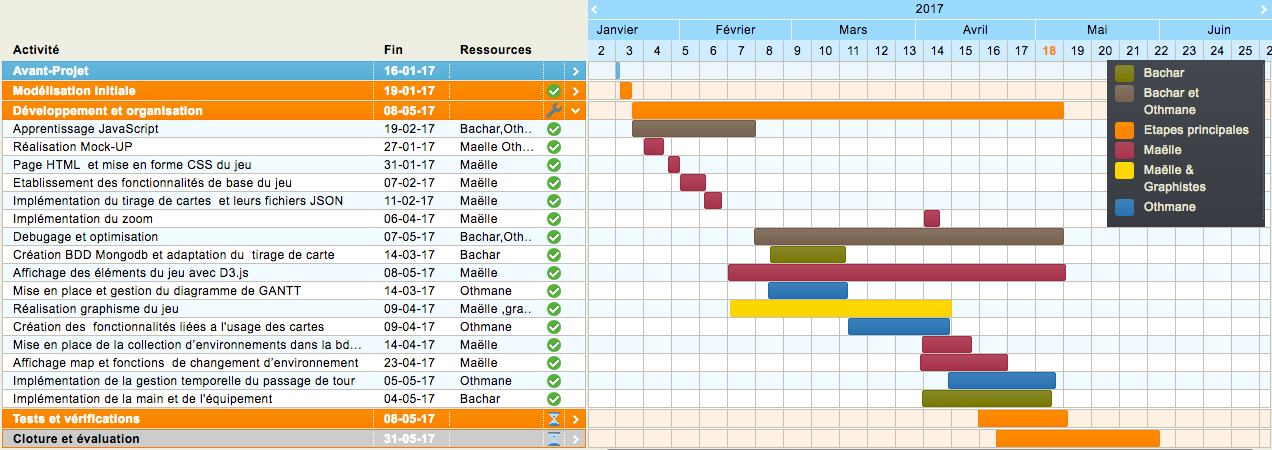
\includegraphics[scale=0.4]{images/diagrammeGantt.jpg}
	    \caption{Diagramme de Gantt du projet}
	    \label{fig:diagGantt}
    \end{figure}

		\newpage
		Ainsi on peut voir sur le diagramme de Gantt sur lequel nous nous sommes appuyés (figure \ref{fig:diagGantt}) quatre activités principales incluant l’étape d’initialisation d’ouvrage précédemment explicitée (avant projet et modélisation initiale).

		Les activités principales du projet étant le développement et l'organisation (voir figure \ref{fig:diagGantt}), nous les avons accompagnées d’un listing de sous-tâches à accomplir qui nous permettait d’avoir une vision synthétique du déroulement du projet.

		Nous nous sommes réparti les tâches et nous sommes réunis chaque semaine avec l'encadrant afin de faire le point sur l'avancement du projet, les éventuelles difficultés et les modifications à apporter. 

		\section{Choix des outils de développement}
		Lorsque l’on travaille à plusieurs sur un projet informatique, on est confronté à plusieurs problèmes liés aussi bien à l’organisation qu’à la compatibilité.
		Pour éviter d'être confrontés à ce genre de problèmes, nous avons utilisé divers outils lors du développement de notre projet.

			\subsection*{Git}
	 		Parmi ces outils, nous avons eu recours à un gestionnaire de versions. Les logiciels de ce type permettent  de stocker un ensemble de fichiers tout en conservant la chronologie de toutes les modifications qui ont été effectuées dessus.
	 		En plus de conserver l’historique d’évolution du code source, cet outil permet de faciliter la collaboration au sein d’un même projet. Et cela en permettant, par exemple, de fusionner les modifications sur un même fichier source sans perte d’information.

	 		Entre les différents gestionnaires de versions disponibles, notre choix s’est porté sur Git qui a l’avantage d’être disponible sur la plupart des systèmes Unix et Windows, mais aussi et surtout d’être de type distribué. Cela signifie que le dépôt de fichier n’est pas unique mais que chaque développeur possède son propre dépôt.

 			\subsection*{Github}
   		L’une des particularités de Git est l’existence de sites web collaboratifs basés sur ce dernier.\\* Parmi ces sites figure GitHub dont nous nous sommes servis tout  au long du projet.
   		GitHub fournit le serveur où les développeurs qui utilisent Git peuvent publier leurs projets ainsi que communiquer et signaler les problèmes de code.

 			\subsection*{Atom}
   		Afin de développer dans les meilleures conditions, il nous semblait préférable d’utiliser le même éditeur de texte.
   		Et dans ce contexte, nous avons choisi unanimement d’utiliser Atom qui fait aussi partie des projets développés  par Github.\\*
   		Outre le fait qu’il soit un logiciel multiplateformes, Atom se distingue par son côté personnalisable.
   		Cet éditeur a été donc l’idéal pour notre projet, surtout en considérant le fait qu’il repose sur le moteur de Node.js, technologie que nous avons utilisée dans le développement de ce projet.


\chapter{Conception}

	Avant de commencer la phase d'implémentation, nous avons modélisé nos objets et préparé une maquette visuelle de notre programme. Nous avons également choisi les technologies nécessaires et pertinentes pour notre projet.

  \section{Modélisation des objets}
	Le jeu se déroulant dans le cadre d'une interaction continue entre les joueurs d'une part, et entre chaque joueur et l'ensemble des cartes tirées depuis la pile et éventuellement stockées dans sa main d'une autre part, nous avons choisi de définir un objet (au sens du JavaScript, c'est à dire un prototype) bien spécifique pour chacune de ces deux entités (joueur et carte).

	En effet, un joueur est identifié par un unique pseudo/alias (une chaîne de caractères), et par un numéro initialisé à -1 quand le joueur n'est pas connecté au jeu, prenant plus tard une valeur entre 0 et 4 une fois connecté au jeu selon son emplacement dans la liste des participants. Par ailleurs, un joueur possède aussi les propriétés descriptives suivantes : les statistiques de défense et d'attaque (des nombres), le statut indiquant l'état de son tour (0 pour non-active et 1 pour active), l'ensemble des cartes dans sa main (un tableau de cartes), et le nombre de cartes équipées.

	D'autre part, une carte est identifiée par un code fantastique, et possède les propriétés descriptives suivantes sous forme de chaînes de caractères : un type (indique si la carte est utilisable, équipable, déclenche un événement, ou une rencontre avec un monstre) une catégorie (éventuellement vide si les cartes ne sont ni utilisables ni équipables, indique la nature de la carte dans le cas contraire, une potion ou une armure par exemple), un chemin (le chemin de l'image depuis l'emplacement du projet), une action (indique l'effet de la carte sous forme d'une fonction ayant un nom et éventuellement des paramètres), et un booléen indiquant si la carte est équipée ou non.

	Outre ces deux objets, nous avons aussi défini un objet pour chaque hexagone de la carte du jeu. En effet, chaque hexagone cartographique est identifié par un code "x:y" dénotant ses coordonnées sur la carte, et possède les propriétés descriptives suivantes (chaînes de caractères) : un environnement indiquant le type du plan dans lequel se déroule le jeu tel qu'une rivière par exemple, et un chemin indiquant l'emplacement de l'image du fond correspondant à l'environnement.

	Enfin, voici le diagramme d'UML représentant les trois objets ci-dessus (voir figure \ref{fig:UML})

	\begin{figure}
		\begin{tikzpicture}
			\umlclass{Player}{
				-- aliasName : String \\
				-- playerNum : String \\
				-- attack : Number \\
				-- defense : Number \\
				-- status : Number \\
				-- nbEquippedCards : Number
			}
			{}
			\umlclass[x=10]{Card}{
				-- id : String \\
				-- type : String \\
				-- category : String \\
				-- path : String \\
				-- action : String \\
				-- isEquipped : boolean
			}
			{}
			\umlclass[x=5.3, y=-4]{MapTile}{
				-- id : String \\
				-- environment : String \\
				-- background : String \\
			}
			{}
			\umluniaggreg[stereo=posséder, mult1=1, arg2=hand, mult2=0..5]{Player}{Card}
		\end{tikzpicture}
		\caption{Diagramme UML}
		\label{fig:UML}
	\end{figure}

  \section{Maquette graphique}
  Afin de visualiser le rendu de notre jeu et avoir une référence lors du code de l'affichage, nous avons réalisé une maquette graphique de notre programme (voir figure \ref{fig:maquette}). Les illustrations n'étant pas encore réalisées à cette étape, nous avons utilisé d'autres dessins d'une artiste collaborant avec nous. Le but de cette maquette n'étant pas de définir l'aspect final mais l'emplacement des objets, elle est minimaliste et le rendu final du jeu devait être plus esthétique.

  \begin{figure}[h!]
  	\centering
    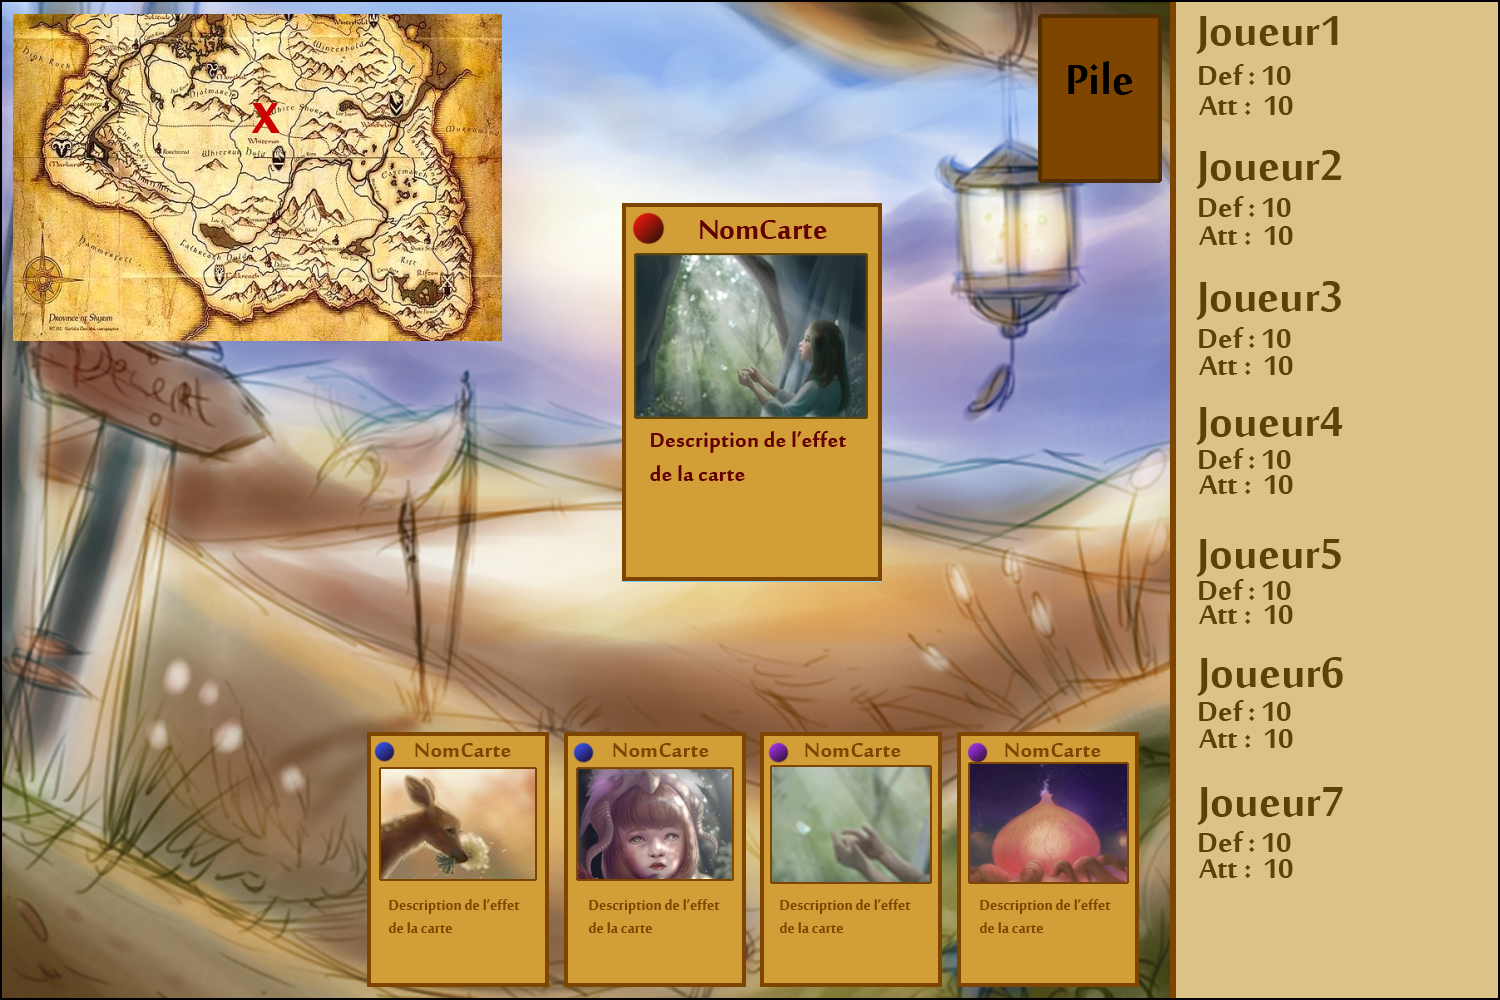
\includegraphics[scale=2.6]{images/mock-up.png}
    \caption{Maquette graphique du jeu.}
    \label{fig:maquette}
  \end{figure}

  \section{Choix des technologies}
	Avant de choisir les technologies permettant une implémentation optimale de notre jeu, nous nous sommes penchés tout d'abord sur l'analyse des contraintes de qualité à satisfaire afin d'assurer un déroulement souple de ce dernier. Autrement dit, nous nous sommes aperçus de la nécessité d'établir une communication en temps réel entre les clients utilisant l'application pour assurer un déroulement réaliste et interactif du jeu, aussi bien que du caractère indispensable du paradigme événementiel pour le rendre plus ergonomique et dynamique. De plus, vu qu'il s'agit d'un jeu, en particulier d'un jeu de société, l'intégration des effets graphiques pour l'animer et le rendre le plus élégant possible paraît évident, voire même trivial.

	Ainsi, pour assurer la réalisation de ces contraintes, nous avons choisi JavaScript comme seul langage de programmation pour développer notre jeu ce qui a plus ou moins réduit la durée de notre apprentissage. Effectivement, l'abondance des fonctionnalités fournies par ce langage permet une implémentation JavaScript pure englobant la totalité de l'architecture client-serveur de notre jeu. En réalité, JavaScript a progressé d'un langage web objet/événementiel incontournable conçu pour la dynamisation des pages web du côté client (manipulation du DOM (\textit{Document Object Model}), la bibliothèque jQuery) en un véritable outil omnipotent avec l'arrivée de NodeJS. En réalité, le modèle non-bloquant avec les fonctions de \textit{callback} caractérisant NodeJS permet une communication extrêmement rapide sur un thread unique entre le serveur et les clients.

	NodeJS intègre aussi la technologie WebSocket dans le module socket.io. Il s'agit d'une API (\textit{Application Programming Interface}) JavaScript permettant un échange bilatéral synchrone entre les clients et le serveur, contrairement aux serveurs web classiques tels que Apache où la communication se déroule normalement d'une façon asynchrone. Cette caractéristique de WebSocket la rend idéale pour des applications nécessitant une communication en temps réel entre les clients comme la nôtre.

	Outre cela, l'API JavaScript D3 offre une myriade de fonctionnalités permettant la mise en \oe{}uvre d'animations, entre autres, notamment avec des éléments SVG, ce qui la rend parfaite pour assurer le respect de la contrainte de qualité relative à l'aspect esthétique du jeu.

  \section{Base de données}
	Pour stocker les cartes, ainsi que les différentes données cartographiques du jeu, nous nous sommes servis de la notation JSON (\textit{JavaScript Object Notation}), un concept fondamental dans le cadre du JavaScript et un moyen très efficace pour la manipulation, le transfert, et le stockage des données.

	Par conséquent, nous avons utilisé le SGBD (Système de Gestion de Bases de Données) offert par MongoDB qui s'avère bien pratique dans le cadre d'une architecture de développement purement basée sur JavaScript telle que la nôtre. En effet, NodeJS offre un module contenant une multitude de fonctionnalités permettant d'interagir aisément avec les bases de données gérées par MongoDB, ce qui facilite énormément la connexion à la base de données et la manipulation des données qui y sont stockées.

	MongoDB permet la création de plusieurs bases de données regroupant chacune les données sous forme de \textit{collections} (concept approximatif équivalent à la notion de \textit{tables} dans le cadre d'un modèle de base de données relationnelle), contenant chacune des \textit{documents} désignant les objets JSON reflétant nos données.

	MongoDB n'utilise pas le langage de requêtes SQL pour gérer les interactions avec la base de données. Toutefois, le langage de requêtes utilisé reste bien facile à maîtriser et puissant pour couvrir une grande gamme de fonctionnalités nécessaires pour une gestion efficace des données.

	Par conséquent, nous avons créé une base de données dans laquelle nous avons stocké nos données en deux collections: une pour stocker les cartes, et l'autre pour stocker les données cartographiques. (voir figure \ref{fig:schemaBDD})

	\begin{figure}
		\centering
		\begin{tikzpicture}[node distance=6.5cm]
		  \node[entity] (card) {Card};
		  \node[attribute] (id) [above=of card] {\underline{Id}} edge (card);
		  \node[attribute] (type) [above right=of card] {Type} edge (card);
			\node[attribute] (category) [above left=of card] {Category} edge (card);
			\node[attribute] (path) [below right=of card] {Path} edge (card);
			\node[attribute] (action) [below left=of card] {Action} edge (card);

		  \node[entity] (maptiles) [right=of card] {MapTiles};
			\node[attribute] (id) [above=of maptiles] {\underline{Id}} edge (maptiles);
		  \node[attribute] (environment) [below right=of maptiles] {Environment} edge (maptiles);
			\node[attribute] (background) [below left=of maptiles] {Background} edge (maptiles);
		\end{tikzpicture}
		\caption{Modèle EA}
		\label{fig:schemaBDD}
	\end{figure}

	\section{Cas d'usage}
	Pour clarifier et résumer tout ce qui vient d'être mentionné, voici deux exemples de cas d'usage permettant de visualiser la progression du jeu selon les actions du joueur :

	  	\subsection{Connexion au jeu et chargement de la carte}
			Avant qu'un joueur puisse tirer une carte, il doit se connecter au serveur. Une fois connecté, sa fenêtre enverra un événement "état" sans aucune donnée et le serveur répondra en lui renvoyant un événement ayant le même nom avec le nombre de joueurs connectés ainsi que leurs noms (ceci même avant qu'il essaie de rejoindre le jeu, donc en mode spectateur). À la réception de l'événement "état" du côté serveur, la fenêtre du client affichera les noms des joueurs ainsi que leurs statistiques d'attaque et de défense. (flèches 1 et 2 en bleu dans figure \ref{fig:useCase1})

			Simultanément, une fois la fenêtre complètement chargée, elle envoie un événement "loadMap" au serveur tout en initialisant les composants de la fenêtre permettant d'afficher et de manipuler la carte du jeu. À la réception de "loadMap", le serveur se connecte à la base de données et récupère la carte qu'il envoie à la fenêtre du joueur avec l'événement "mapLoaded". Suite à la réception de "mapLoaded" la fenêtre du joueur stocke la carte du jeu et l'affiche dans la fenêtre du jeu. (flèches 1, 2, 3 et 4 en orange dans figure \ref{fig:useCase1})

			Le joueur essaie après de rejoindre le jeu en saisissant un pseudo (qui doit être unique parmi les pseudos des participants) dans la région de saisie dans sa fenêtre puis en cliquant sur le bouton "Rejoindre l'aventure". Une fois le clic effectué, le bouton envoie l'événement "rejoindre" joint par un objet encapsulant le pseudo du joueur. Une fois le serveur reçoit l'événement "rejoindre" il crée une nouvelle instance de l'objet "Player", tout en initialisant les propriétés du nouveau joueur comme il faut (l'attribution des statistiques de base pour la défense et l'attaque, un tableau vide correspondant à une main vide, l'initialisation du tour du nouveau joueur en fonction des joueurs connectés, la mise à jour du nombre des joueurs connectés, etc...). Après, le serveur renvoie deux événements : "newPlayer" avec les propriétés initialisées du joueur et "status" avec le statut du tour du joueur.

			À la réception de "newPlayer", la fenêtre du nouveau joueur affichera les informations du nouveau joueur. À la réception de "status", le tour du nouveau joueur sera initialisé selon le nombre de joueurs participants. Si c'est le premier joueur connecté, cela sera directement à son tour de tirer une carte, sinon son tour sera activé une fois que le joueur le précédant dans la liste des joueurs aura joué. (flèches 3 et 4 en bleu dans figure \ref{fig:useCase1})

			\begin{figure}[h!]
		  	\centering
		    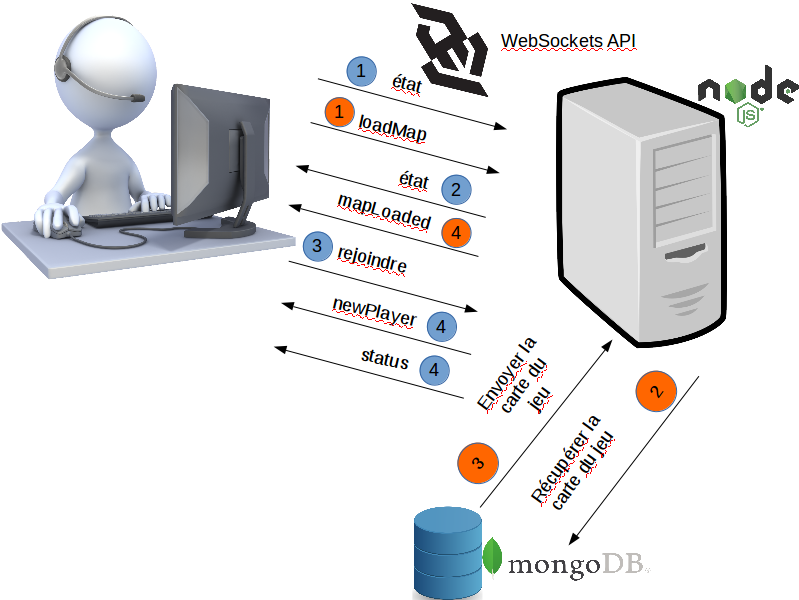
\includegraphics[scale=0.5]{images/useCase1.png}
		    \caption{Connexion au jeu et chargement de la carte.}
				\label{fig:useCase1}
		  \end{figure}

			\subsection{Tirage et utilisation d'une carte utilisable de catégorie potion}
			Après la connexion au jeu et l'affichage de la carte du jeu, le joueur attend son tour pour pouvoir tirer une carte depuis la pile. Une fois son tour activé, le joueur aura la possibilité de cliquer sur la pile de cartes et/ou manipuler les cartes de sa main avant de faire passer son tour au joueur suivant en cliquant sur le bouton "Terminer le tour". Si le joueur ne clique pas sur le bouton pendant une minute après avoir interagit avec le jeu, son tour sera passé automatiquement au joueur suivant.

			Dans le délai d'une minute, le joueur clique sur la pile des cartes et l'événement "drawCard" sera envoyé au serveur sans aucune donnée. À la réception de "drawCard", le serveur se connecte à la base de données et récupère aléatoirement une carte depuis l'ensemble des cartes stockées. Une fois la carte récupérée, le serveur envoie l'événement "showCard" avec la carte tirée à tous les joueurs pour que leurs fenêtres correspondantes puissent l'afficher. Simultanément, le serveur envoie l'événement "drawCard" avec la carte tirée au joueur qui a tiré la carte pour activer les boutons permettant de la prendre ou de la défausser. (voir figure \ref{fig:useCase21})

			\begin{figure}[h!]
		  	\centering
		    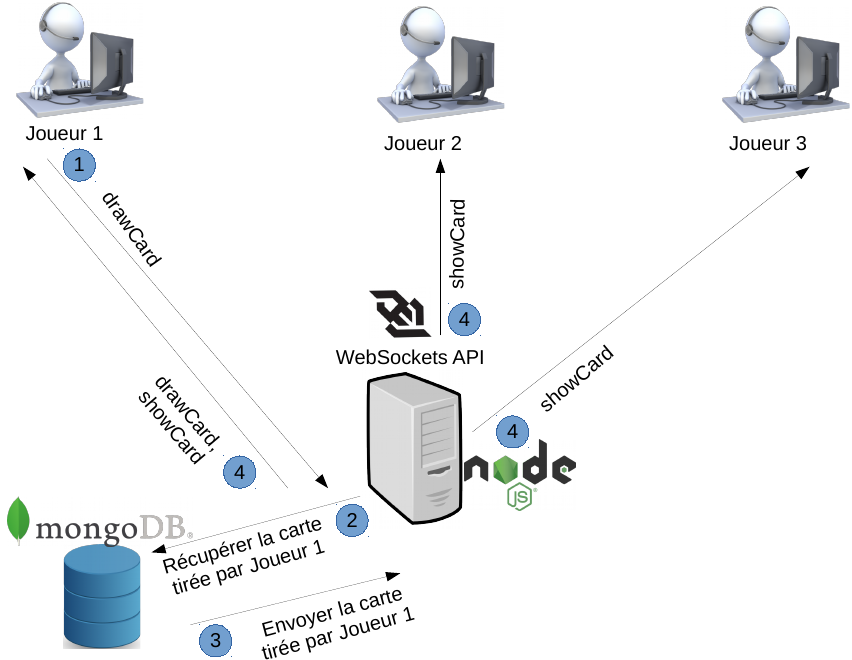
\includegraphics[scale=0.5]{images/useCase21.png}
		    \caption{Tirage et affichage d'une carte.}
				\label{fig:useCase21}
		  \end{figure}

			À la réception de l'événement "showCard", les fenêtres de tous les joueurs participants affichent la carte tirée. D'autre part, à la réception de l'événement "drawCard", le joueur aura la possibilité de choisir entre prendre la carte ou de la défausser si c'est une carte utilisable/équipable, sinon la carte sera un événement ou un monstre.

			Dans cet exemple la carte tirée est de type utilisable. En particulier il s'agit d'une carte correspondant à une potion que le joueur choisit de prendre en cliquant sur le bouton "Prendre" qui sera affiché sur sa fenêtre une fois la carte tirée. En cliquant sur le bouton "Prendre", le statut d'équipage de la carte sera mis à faux, la carte sera stockée dans la main du joueur local, la main du joueur local sera affichée, et puis l'événement "cardTaken" sera envoyé au serveur.

			L'événement "cardTaken" est envoyé pour mettre à jour les données du joueur sur le serveur et puis l'événement "discardCardAllClients" sera envoyé par le serveur à tous les joueurs pour enlever la carte affichée au sein de la fenêtre du jeu. (voir figure \ref{fig:useCase22})

			\begin{figure}[h!]
		  	\centering
		    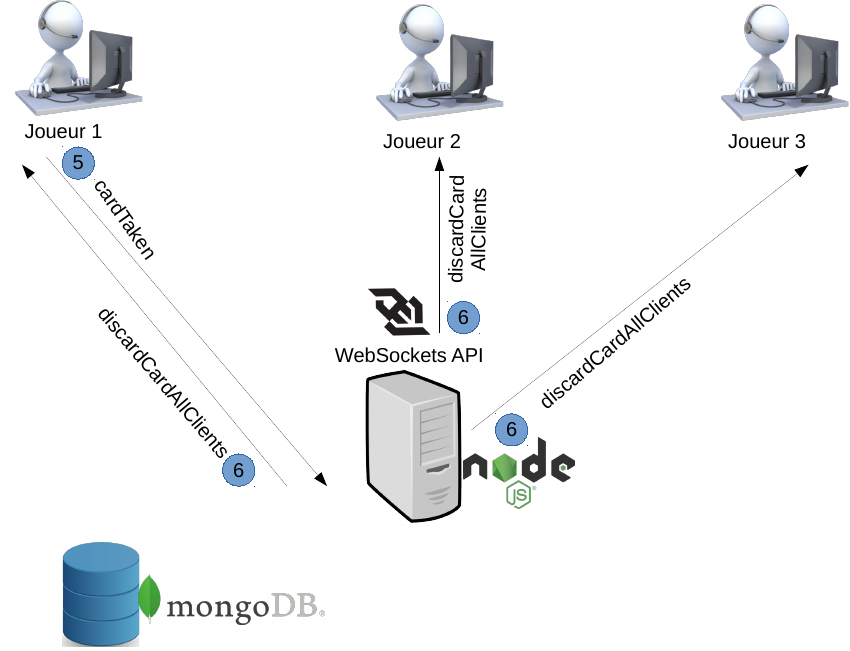
\includegraphics[scale=0.5]{images/useCase22.png}
		    \caption{Prendre une carte tirée et l'enlever depuis la fenêtre du jeu de tous les joueurs.}
				\label{fig:useCase22}
		  \end{figure}

			Lorsque la main du joueur local est affichée, il aura la chance de survoler chaque carte avec le curseur de la souris pour zoomer dessus et voir son effet. De plus, le joueur pourra cibler une carte pour la manipuler (soit l'utiliser en tapant sur la touche "u" ou "U", soit la défausser en appuyant sur la touche "t" ou "T", soit l'équiper, si elle est équipable, en tapant sur la touche "e" ou "E").

			Dans cet exemple, comme indiqué précédemment, la carte tirée est une potion que le joueur souhaite prendre. Le joueur cible ainsi la carte et appuie sur la touche "u" engendrant l'exécution de l'action associée à la carte, l'envoi de l'événement "modifyCard" au serveur, le retrait de la carte de la main du joueur, et le nouvel affichage de la main par la suite.

			L'exécution de l'action associée à la carte modifie les statistiques du joueur local et envoie l'événement "modify" au serveur pour refléter les changements locaux au sein du serveur. Une fois les modifications effectuées, le serveur envoie les nouvelles valeurs des statistiques à tous les joueurs pour les afficher localement sur leurs fenêtres de jeu correspondantes grâce à l'événement "état". D'autre part, l'événement "modifyCard" est envoyé pour enlever la carte depuis la main du joueur au sein du serveur. (voir figure \ref{fig:useCase23})

			\begin{figure}[h!]
		  	\centering
		    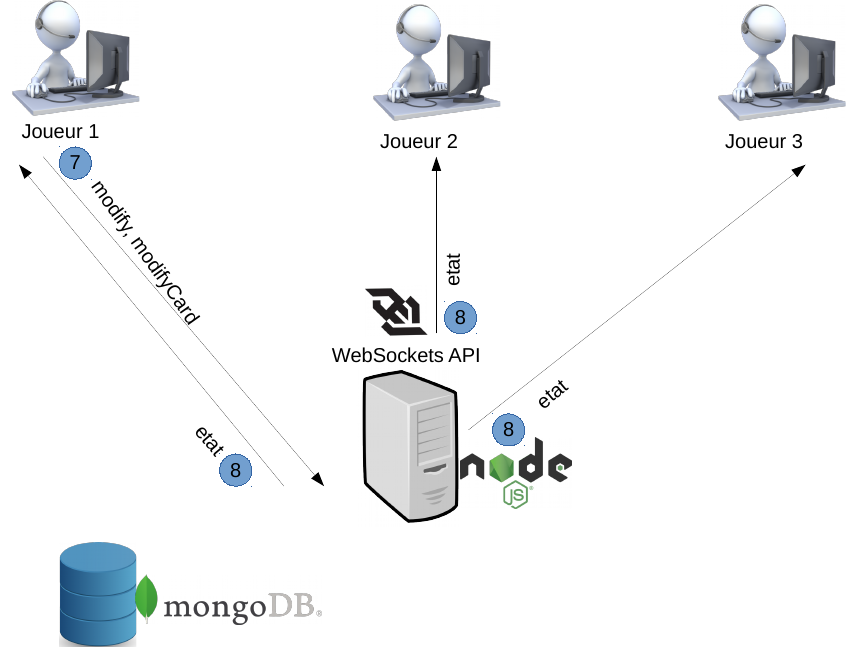
\includegraphics[scale=0.5]{images/useCase23.png}
		    \caption{Utiliser une carte dans la main et mettre à jour les statistiques du joueur.}
				\label{fig:useCase23}
		  \end{figure}

			Une fois que le joueur a terminé son tour il aura la possibilité de cliquer sur le bouton "Terminer le tour" ou d'attendre la fin du délai d'une minute pour envoyer l'événement "playerTurn" au serveur afin d'activer le tour du joueur suivant. À la réception de l'événement "playerTurn" le serveur activera le tour du joueur suivant et enverra l'événement "status" à tous les joueurs de la partie pour les informer de l'identité du joueur suivant. (voir figure \ref{fig:useCase24})

			\begin{figure}[h!]
		  	\centering
		    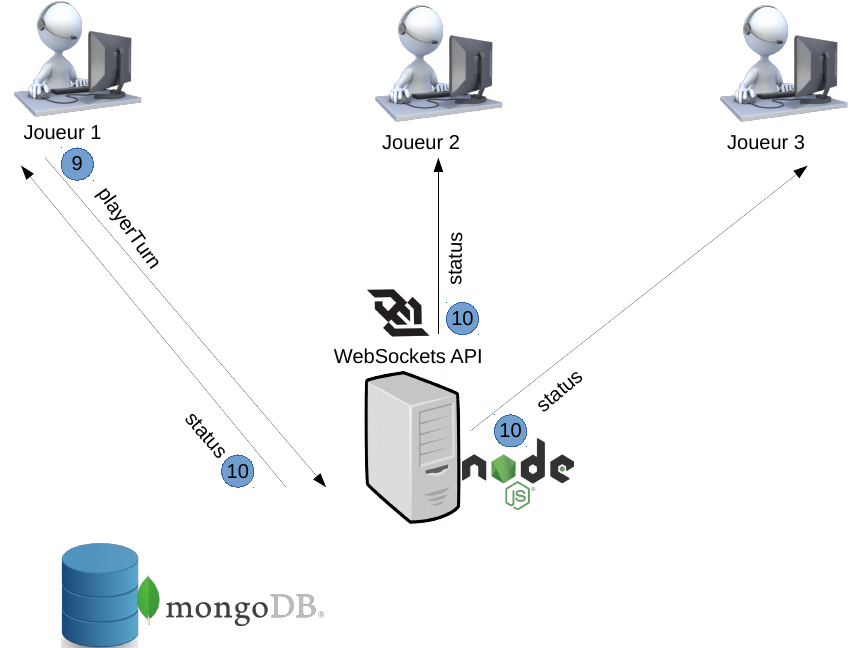
\includegraphics[scale=0.5]{images/useCase24.png}
		    \caption{Faire passer le tour au joueur suivant.}
				\label{fig:useCase24}
		  \end{figure}

\chapter{Développement}

  \section{Gestion de l'événementiel}
	L'un des atouts de la programmation événementielle est qu'elle ajoute un dynamisme à l'application en se basant sur une modélisation intuitive de la gestion des événements et de leurs fonctions de rappel correspondantes (\textit{callback functions} ou \textit{handlers}). Celle-ci consiste à rendre l'interaction entre les utilisateurs et l'application comme la source principale influençant la progression de l'application et sa transition entre les différents états du programme.

	En particulier, ce paradigme est caractéristique du langage JavaScript et de toutes les API et \textit{frameworks} qui sont basés dessus. Dans notre jeu nous avons utilisé différentes façons d'implémenter cette interaction selon le cas d'utilisation. En effet, pour gérer les événements dont les fonctions de \textit{callback} avaient uniquement un effet local sur la fenêtre du client, nous nous sommes servis des fonctionnalités offertes par l'API JavaScript permettant de manipuler le DOM, de la bibliothèque jQuery, et de l'API D3 pour les effets graphiques. D'autre part, pour gérer les événements dont les fonctions de \textit{callback} avaient des effets qui doivent être transmises au serveur, et éventuellement du serveur aux clients par la suite, nous avons utilisé les fonctionnalités offertes par le module socket.io.

	L'implémentation de la gestion des événements à travers l'API de JavaScript pour manipuler le DOM se fait de la manière suivante:

	\begin{verbatimtab}[4]
		element.addEventListener(event, function(params){
			//actions
		});
	\end{verbatimtab}

	\begin{description}
		\item[element :]{
			un objet désignant un élément du DOM
			(un bouton ayant la balise <button> par exemple en HTML).
		}
		\item[event :]{
			une chaîne de caractères désignant un événement
			(click, keypress, focus, etc...).
		}
		\item[params :]{
			les éventuels paramètres utilisés par la fonction de rappel dans son corps
			(e par exemple pour désigner l'événement associé à la fonction).
		}
	\end{description}

	L'implémentation de la gestion des événements à travers la bibliothèque jQuery se fait de la manière suivante:

	\begin{verbatim}
		$(css_selector).on(event, function(params){
		  //actions
		});
	\end{verbatim}

	\begin{description}
		\item[\$ :]{
			l'objet parent de la bibliothèque jQuery permettant de sélectionner les éléments de la page web.
		}
		\item[css\_selector :]{
			un sélecteur css permettant de récupérer un ou plusieurs éléments de la page web.
		}
		\item[event :]{
			idem que \textbf{event} dans l'exemple avec l'API JavaScript pour manipuler le DOM.
		}
		\item[params :]{
			idem que \textbf{params} dans l'exemple avec l'API JavaScript pour manipuler le DOM.
		}
	\end{description}

	L'implémentation de la gestion des événements à travers le module socket.io se fait de la manière suivante:

	\begin{verbatimtab}[4]
	/*CLIENT*/

	//pour émettre un événement personnalisé au serveur avec éventuellement
	//des données

	socket.emit(customizedClientEvent, clientData);

	//pour lancer une fonction de rappel en réception d'un événement
	//personnalisé du serveur

	socket.on(customizedServerEvent, function(serverData){
		//actions
	});

	/*SERVEUR*/

	//émettre un signal à tous les clients avec éventuellement des données

	io.emit(customizedServerEvent, serverData);

	//émettre un signal à un client suite à la réception d'un événement
	//envoyé par ce dernier

	socket.on(customizedClientEvent, function(clientData){
		//actions
		socket.emit(customizedServerEvent, serverData);
		//actions
	});

	//suite à la réception d'un événement d'un client,
	//émettre un signal à tous les autres clients

	socket.on(customizedClientEvent, function(clientData){
		//actions
		socket.broadcast.emit(customizedServerEvent, serverData);
		//actions
	});
	\end{verbatimtab}

	\begin{description}
		\item [socket :]{
			l'objet désignant le socket permettant la communication en temps réel entre le client et le serveur.
		}
		\item [customizedClientEvent :]{
			une chaîne de caractères désignant le nom d'un événement personnalisé émis par le client ("drawCard", "drawMap" par exemple).
		}
		\item [clientData :]{
			un éventuel objet contenant des données que l'on souhaite faire passer au serveur.
		}
		\item [customizedServerEvent :]{
			une chaîne de caractères désignant le nom d'un événement personnalisé émis par le serveur.
		}
		\item [serverData :]{
			les éventuelles données envoyées par le serveur sous forme d'un objet.
		}
	\end{description}

	Dans notre jeu, nous avons utilisé ces trois manières différentes pour gérer les événements que nous avons catégorisés en trois grande parties:
	\begin{enumerate}
		\item{Connexion au serveur, joindre et quitter le jeu;}
		\item{Chargement et affichage de la carte du jeu;}
		\item{Manipulation des cartes du jeu.}
	\end{enumerate}

  \section{Graphismes}
	Aidés par les artistes avec lesquels nous avons collaboré, nous avons entièrement réalisé les graphismes de notre jeu, avant d'implémenter l'affichage de ceux-ci. Un travail collaboratif donc, que nous allons détailler dans cette partie.

    \subsection{Réalisation des images}
		Afin d'obtenir un rendu esthétique pour le jeu, nous avons créé des illustrations avec l'aide des illustrateurs avec lesquels nous avons collaboré. Ceux-ci se sont chargés de faire les fonds pour les environnements plaine et rivière, ainsi que les deux épées présentes sur les cartes du jeu.

    \begin{figure}[h!]
     	\centering
       	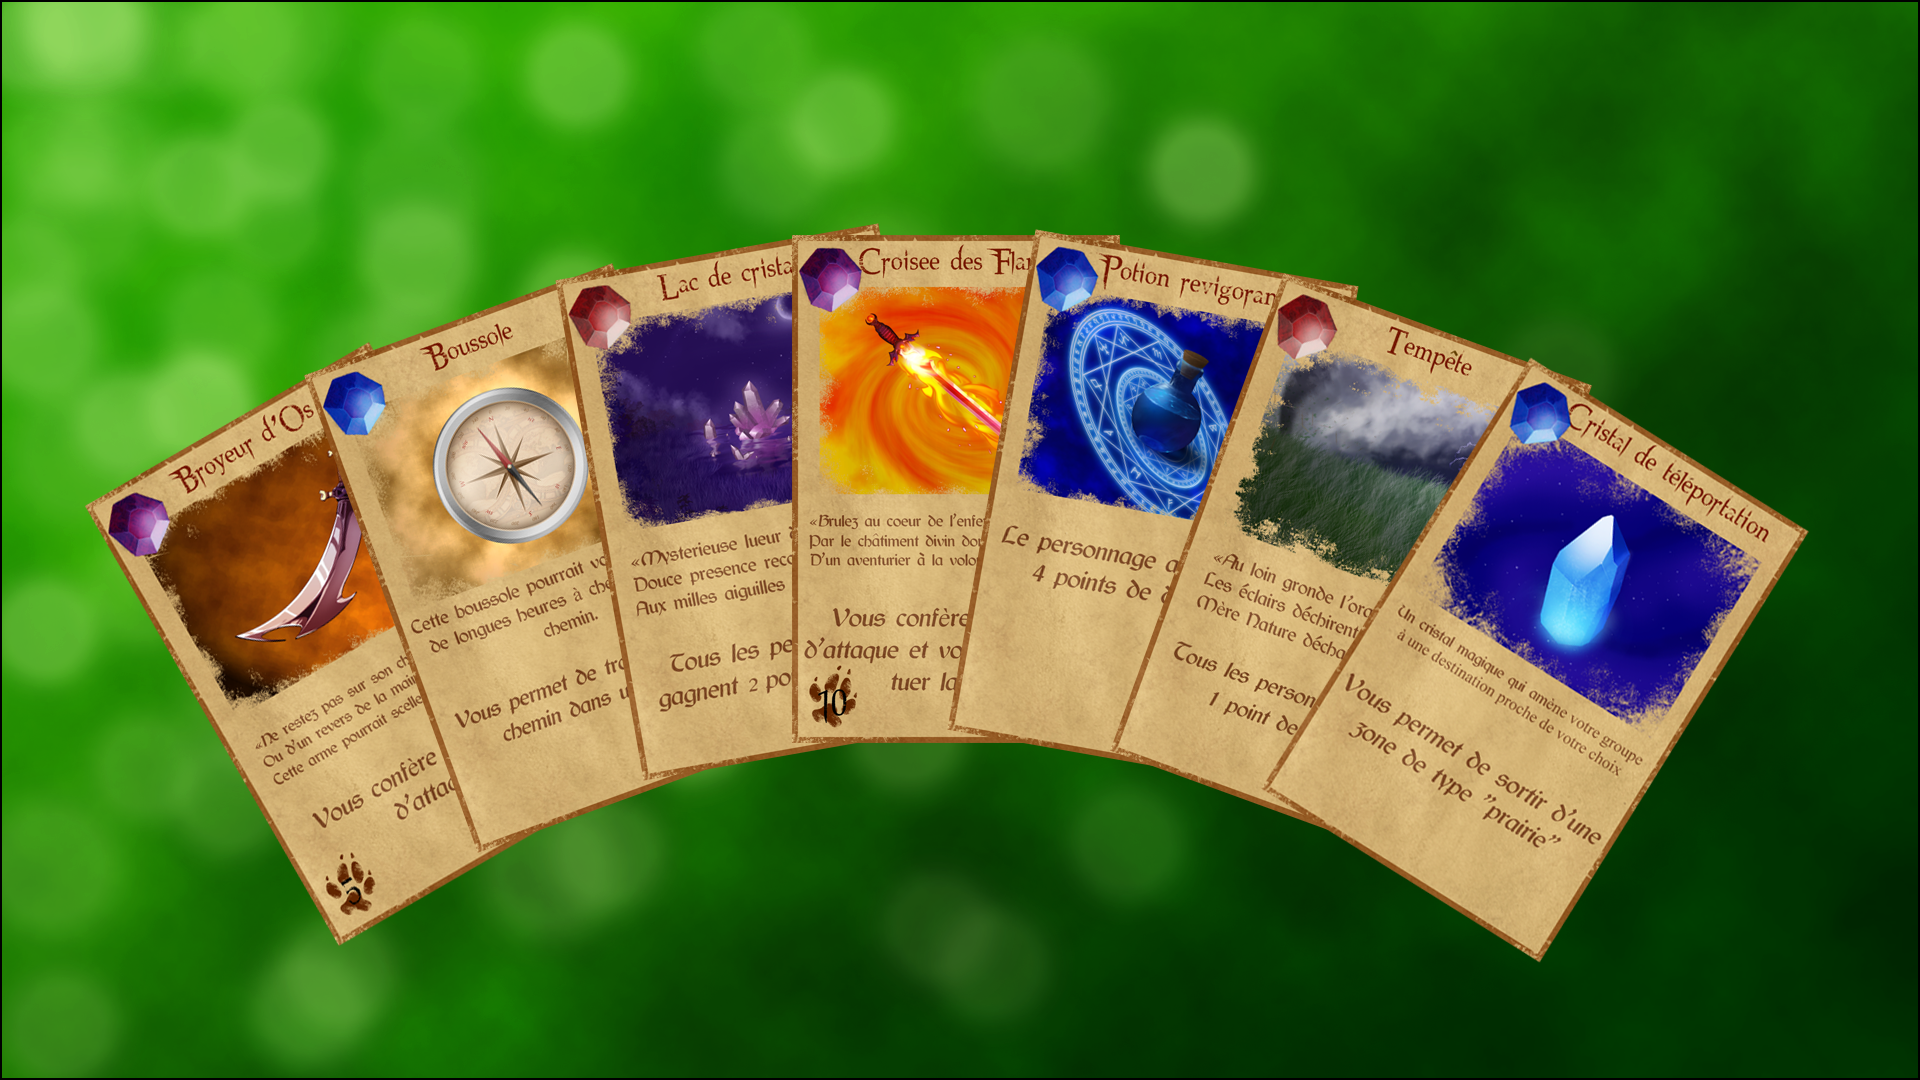
\includegraphics[scale=0.45]{images/cards.png}
       	\caption{Exemple de cartes crées ainsi que le fond du site.}
       	\label{fig:cartes}
    \end{figure}

    Nous nous sommes chargés de réaliser, à l'aide d'un logiciel de dessin assisté, les autres illustrations pour les cartes, les éléments de décoration des cartes (gemme indiquant le type, symboles d'attaque et de défense, effets visuels... Voir figure \ref{fig:cartes}), le fond pour l'environnement "forêt", le dos de carte pour la pile, ainsi que les autres éléments décoratifs du site (texture de bois, fond).

    Chaque illustration nous a demandé plusieurs heures de travail, et il était prévu que nos collaborateurs réalisent la majeure partie des graphismes. Cependant, par manque de temps de leur part, nous avons dû investir plus de temps que prévu dans cette partie du projet.

    \subsection{Affichage graphique en JavaScript}
		Pour afficher les différents éléments du jeu (cartes de jeu, pile, carte de la zone) nous avons utilisé la bibliothèque D3. Celle-ci permet de manipuler des éléments SVG (\textit{Scalable Vector Graphics}, format d'images vectorielles).

    Nous avons créé une zone SVG recouvrant toute la partie du site dédiée au jeu, de la manière suivante :

    \begin{verbatim}
    var svg = d3.select('#svgWin')
                .append('svg')
                .attr('width', 900)
                .attr('height', 650);
    \end{verbatim}

    Ici, 'svgWin' désigne la balise html \textless{}div\textgreater{} ayant pour attribut "id = 'svgWin' ". La fonction append('svg') permet de créer un élément SVG fils de "svgWin". Nous lui attribuons ensuite une largeur et une hauteur correspondant à la taille de la zone dédiée au jeu. Nous avons procédé de la même manière pour les images, avec des objets de type "svg:image", en y ajoutant les attributs "x" et "y" pour la position dans la zone SVG.

    Outre l'affichage d'image, nous avons également affiché la carte des zones du jeu à l'aide de D3 (voir figure \ref{fig:map}). Pour cela, nous avons créé des hexagones que nous avons rempli de couleurs correspondant à l'environnement de la zone représentée par chaque hexagone. Le dessin des hexagones est réalisé à l'aide de "path", qui permet de dessiner les contours d'une forme (rectangle, cercle, simple ligne...). Voici un exemple de code simplifié permettant d'afficher plusieurs formes à la suite :

	\begin{verbatim}
for(let l=0; l < lines; l++){
    for(let c=0; c < columns; c++){
        d = "";
        for(h in shape){
            x = // On attribue ici la valeur de l'abscisse en fonction de h
            y = // On attribue ici la valeur de l'ordonnée en fonction de h
            d += // On attribue ici la valeur de d en fonction de x et y
        }
    }

    d3.select(element).append('path')
                      .attr('d', d)
                      .attr('stroke', color)
                      .attr('fill', color2);
}
	\end{verbatim}

	\begin{itemize}
        	\item \textbf{Lines} représente le nombre de lignes sur lesquelles nous voulons afficher les formes.
        	\item De même, \textbf{columns} représente le nombre de colonnes. \item \textbf{color} et \textbf{color2} sont respectivement les couleurs du contour et du remplissage de la forme (l'attribut "stroke" étant le tracé de "path" et "fill" son remplissage). \item \textbf{Element} est l'élément svg auquel nous voulons rajouter les formes à afficher.
        	\item \textbf{Shape} est un tableau de points correspondant à la forme que nous souhaitons dessiner.
        	\item \textbf{d} permet de définir la forme du tracé de "path".
	\end{itemize}

	La position sur la carte, qui se déplace lorsque les joueurs changent de lieu, est marquée par un cercle.

	\begin{figure}[h!]
		\centering
		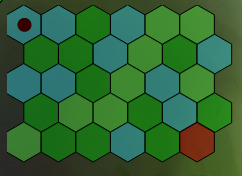
\includegraphics[scale=0.8]{images/map.png}
		\caption{La carte des zones du jeu implémentée en JavaScript (D3)}
		\label{fig:map}
	\end{figure}

    Nous avons également utilisé D3 pour effectuer un zoom sur les cartes en main lors du passage de la souris sur celles-ci (voir figure \ref{fig:zoom}) afin que les joueurs puissent lire les effets de leurs cartes plus facilement.

	\begin{figure}[h!]
		\centering
		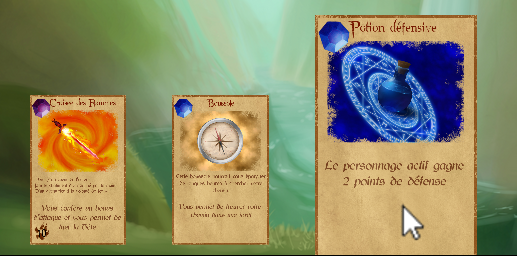
\includegraphics[scale=0.6]{images/zoom.png}
		\caption{Le zoom effectué lorsque la souris est passée sur une carte de la main}
		\label{fig:zoom}
	\end{figure}

\chapter{Manuel d'utilisation}

	\section{Navigation sur le site}

		Le site comporte trois différentes pages (voir figure \ref{fig:ArchiSite}), accessibles depuis la barre de menu en haut (voir figure \ref{fig:manual}). La page principale est celle concernant uniquement le jeu, avec en haut à gauche le champ de texte pour entrer un pseudo et se connecter, ainsi que le bouton permettant de quitter la partie (voir figure \ref{fig:manual}). Au centre de la page se trouve la fenêtre du jeu.

		\begin{figure}[h!]
			\centering
			\begin{tikzpicture}[node distance=1cm, auto]
			\tikzset{
				mynode/.style={rectangle,rounded corners,draw=black, top color=white, bottom color=yellow!50,very thick, inner sep=1em, minimum size=3em, text centered},
				myarrow/.style={->, >=latex', shorten >=1pt, thick},
				mylabel/.style={text width=7em, text centered}
			}
			\node[mynode] (accueil) {Page du jeu/accueil};
			\node[below=3cm of accueil] (dummy) {};
			\node[mynode, left=of dummy] (retailer1) {Règles du jeu};
			\node[mynode, right=of dummy] (retailer2) {Remerciements};

			\draw[myarrow] (accueil.south) -- ++(0,0) -- ++(0,-1) -|
			(retailer1.north);
			\draw[myarrow] (accueil.south) -- ++(0,0) -- ++(0,-1) -|  (retailer2.north);
			\end{tikzpicture}
			\caption{Architecture du site}
			\label{fig:ArchiSite}
		\end{figure}

		Il est possible de consulter les règles du jeu en cliquant sur le lien 	"Règles" dans le menu. On y trouve toutes les informations nécessaires pour une partie.

		Enfin, tous les contributeurs du projet (les artistes ayant collaboré avec nous ainsi que nous-mêmes) sont listés sur la page "remerciements", également accessible à l'aide du lien ayant le même nom dans le menu.

	\section{Fonctionnement du jeu}
		Une fois la partie commencée, chaque joueur joue tour à tour. Un tour consiste à tirer une carte de la pile, en cliquant sur l'image du dos de carte sur la gauche de la fenêtre de jeu (voir figure \ref{fig:manual}). Le joueur peut alors décider de prendre la carte ou la jeter, en cliquant sur le bouton correspondant qui s'affichera en même temps que la carte tirée, qui sera affichée au centre de l'écran (voir figure \ref{fig:manual}).

		Les cartes que le joueur décide de prendre s'affichent en bas de la fenêtre du jeu (voir figure \ref{fig:manual}). La main du joueur est limitée à cinq cartes, par conséquent, si l'on a déjà une main pleine on ne peut pas prendre de nouvelle carte sans se débarrasser d'une autre. Différentes interactions sont possibles avec les cartes que l'on a en main : en cliquant sur une carte, des choix s'offrent à nous. S'il s'agit d'une carte équipable, on peut l'équiper en appuyant sur "e". S'il s'agit d'une carte utilisable (potion ou objet permettant de changer de lieu), on peut l'utiliser en appuyant sur "u". Dans tous les cas, il est possible de jeter la carte en appuyant sur "t" si on décide qu'elle ne nous est plus d'aucune utilité ou que l'on souhaite faire de la place dans notre main.

		\begin{figure}[h!]
			\centering
			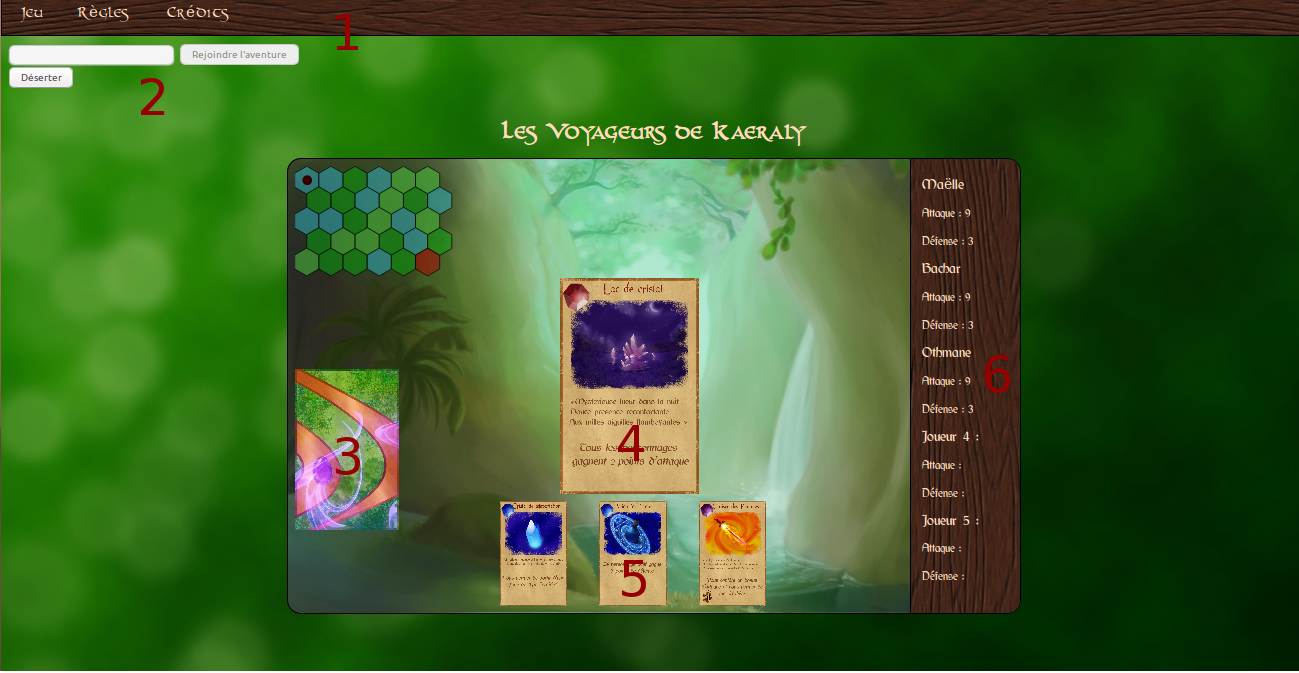
\includegraphics[scale=0.35]{images/manual.png}
			\label{fig:manual}
			\caption{Aperçu de la page du jeu et ses différents éléments.}
		\end{figure}

		La carte en haut à gauche de la zone de jeu permet de savoir où se trouvent les joueurs ainsi que les environnements des différentes zones. Le point représente la position des joueurs. Les zones bleues sont de type "rivière", le vert clair représente les zones "prairie" et le vert foncé l'environnement "forêt". Le fond de la zone de jeu s'accorde à l'environnement dans lequel se trouvent les joueurs.

		Dans le cas de l'utilisation d'un objet permettant de changer de zone, il faut choisir la zone suivante dans laquelle les joueurs veulent se placer. Il est impossible de reculer, seules trois directions sont possibles : haut, droite, bas.

		Un joueur dispose d'un temps imparti pour terminer son tour. Il est possible de passer son tour après avoir réalisé toutes les actions que l'on souhaitait faire en cliquant sur le bouton "Terminer le tour". Si le joueur ne clique pas sur ce bouton dans le temps, le tour passe automatiquement au joueur suivant afin d'éviter que la partie ne soit bloquée par un joueur inactif.

		Les cartes équipables ainsi que les potions permettent de modifier les statistiques de défense et/ou d'attaque d'un joueur. Celles-ci sont visibles sur le côté droit de la fenêtre du jeu (voir figure \ref{fig:manual}).

\chapter*{Conclusion}
\addcontentsline{toc}{chapter}{Conclusion}

  \section*{Bilan}
  \addcontentsline{toc}{section}{Bilan}
  Globalement, nous avons réussi à développer une version fonctionnelle du jeu. Nous avons implémenté une majeure partie des fonctionnalités que nous souhaitions intégrer au projet. Les mécanismes de base du jeu tels que le tour par tour ou encore le tirage de cartes fonctionnent bien. Les éléments cartographiques sont également terminés et fonctionnels. Nous avons réussi l'affichage graphique de tous les éléments (cartes tirées, cartes équipées, pile, etc) et également les fonctions permettant l'interaction avec les cartes.

  En revanche, il nous reste quelques problèmes à résoudre, certains cas d'erreur et quelques fonctionnalités que nous comptons rajouter avant la fin du temps imparti pour le projet. Parmi ces fonctionnalités, l'affichage des cartes équipées par chaque joueur en passant la souris sur son nom, mais également le combat avec le monstre qui n'est pas encore fonctionnel. Nous avons également manqué de temps pour réaliser le nombre de cartes que nous souhaitions intégrer, notamment car nos coéquipiers illustrateurs ont renoncé à leur rôle au cours du projet par manque de disponibilité.

  \section*{Perspectives}
  \addcontentsline{toc}{section}{Perspectives}
	Nous avons l'intention d'améliorer le jeu en y ajoutant des fonctionnalités afin d'y ajouter plus de stratégie, de dynamisme et d'effets visuels. Par exemple, il serait bien de pouvoir y intégrer un système de classes de personnages : chaque joueur choisirait à sa connexion une classe parmi plusieurs, sachant que certains objets seraient spécifiques à une classe. Nous pourrions également ajouter la possibilité de donner des cartes à un autre joueur afin d'améliorer la coopération du groupe.

  Pour ajouter à l'esthétisme du jeu, nous pourrions intégrer des animations pour le tirage de carte par exemple, ou encore pour le changement de zone. Nous pourrions également accompagner l'effet visuel d'un effet audio avec des bruitages spécifiques à certaines cartes.

  Enfin, nous comptons rajouter des cartes de chaque type afin de diversifier le jeu, ainsi que faire évoluer l'objectif en y intégrant des étapes (par exemple, vaincre un premier monstre, puis obtenir un certain objet, avant de tuer le monstre final).

  \section*{Apports personnels du projet}
  \addcontentsline{toc}{section}{Apports personnels du projet}
  La réalisation de ce projet nous a tout d'abord amenés à apprendre un langage qui jusqu'ici ne nous avait pas été enseigné. Nous avions en effet l'habitude de travailler avec le C ou le C++ et nous avions peu de connaissances en développement web. Nous avons également appris à utiliser NodeJS et notamment les WebSockets, ainsi que la gestion de base de données NoSQL que nous avons abordés pour la première fois en travaillant sur le jeu. L'utilisation de D3 a enrichi les connaissances en JavaScript que nous avons acquises pour développer ce jeu, en nous donnant un aperçu des nombreuses possibilités de cet API.

  Outre les connaissances informatiques, le travail en groupe nous a apporté de l'expérience en gestion de projet, de répartition des tâches et gestion du temps, ainsi qu'en communication et compréhension de l'autre.

  Enfin, nous avons appris les bases de la création d'un projet car nous avons préféré créer notre propre projet plutôt que partir sur un sujet proposé par un encadrant. Il nous a donc fallu établir nous-mêmes le cahier des charges à respecter.

\end{document}
